
\section{Recent UCVM Applications}

This section showcases research efforts where UCVM has been used to facilitate the creation of materialized velocity models, that is, numerical discrete models based on velocity models that can be used in simulations and research in geosciences.

\subsection{The 2008 Chino Hills Case Study}

On 29 July 2008 the region of southern California and in particular, the greater Los Angeles metropolitan area, was struck by a magnitude \eqmag{w} 5.4 earthquake at 11:42 a.m. The earthquake was the strongest felt in the city since the 1994 Northridge earthquake, but caused no significant damages or fatalities. It provided, nonetheless, an excellent opportunity for earthquake studies because its shaking was recorded on a numerous set of monitoring stations. Since then, UCVM and other SCEC initiatives have used the data during this earthquake as a case study for testing different simulation methods and models. Two particular efforts involving the use of the UCVM platform are noteworthy and serve here as application examples of how UCVM is being used to advance research in geoscience.

\subsubsection{Validation studies using different velocity models}

Various recent studies done have carefully conducted validations of simulations of the 2008 Chino Hills earthquake with models created using UCVM \citep[e.g.,][]{Olsen_2010_SRL, Taborda_2013_BSSA, Taborda_2014_BSSA}. They have helped test the simulation capabilities of current modeling approaches to predict the ground motion of moderate magnitude earthquakes at low ($<1$~Hz) and moderately (1--4~Hz) and high ($>4$~Hz) frequencies using deterministic and hybrid methods, as well as to propose and test different validation algorithms (goodness-of-fit criteria). 

The latest of these studies \citep{Taborda_2014_BSSA}, in particular, focuses on the validation of simulations of the Chino Hills earthquake using different velocity models, namely CVM-S and CVM-H. This in turn have helped evaluate the differences between the models and their accuracy. The validation performed in this study is based on comparisons with recorded seismograms in over 300 stations scattered throughout the region. The simulation and the models used created with UCVM cover an area of \adomain{180}{135}{km} and go as deep as 62~km. Figure \ref{fig:ch.validation} shows comparisons between the crustal structures of the two models, results of the surface peak ground velocity obtained from the simulations and contour maps of the validation results. The models created for these simulations were built using the etree MPI utilities on NICS's Kraken and NCSA's Blue Waters supercomputer systems employing between XX and YY thousand cores for up to ZZ hours. The sizes of the output (etree) files range between XXX and XXX GB and they comprised between 5 billion and 15 billion octants. \textcolor{red}{(This paragraph needs to be improved.)}


% ---------------------------------------------------------------------------------------------
% TEMP FIGURE: Needs to be improved in Illustrator and moved to final PDF dir.
\begin{figure*}[ht!]
	\centering
	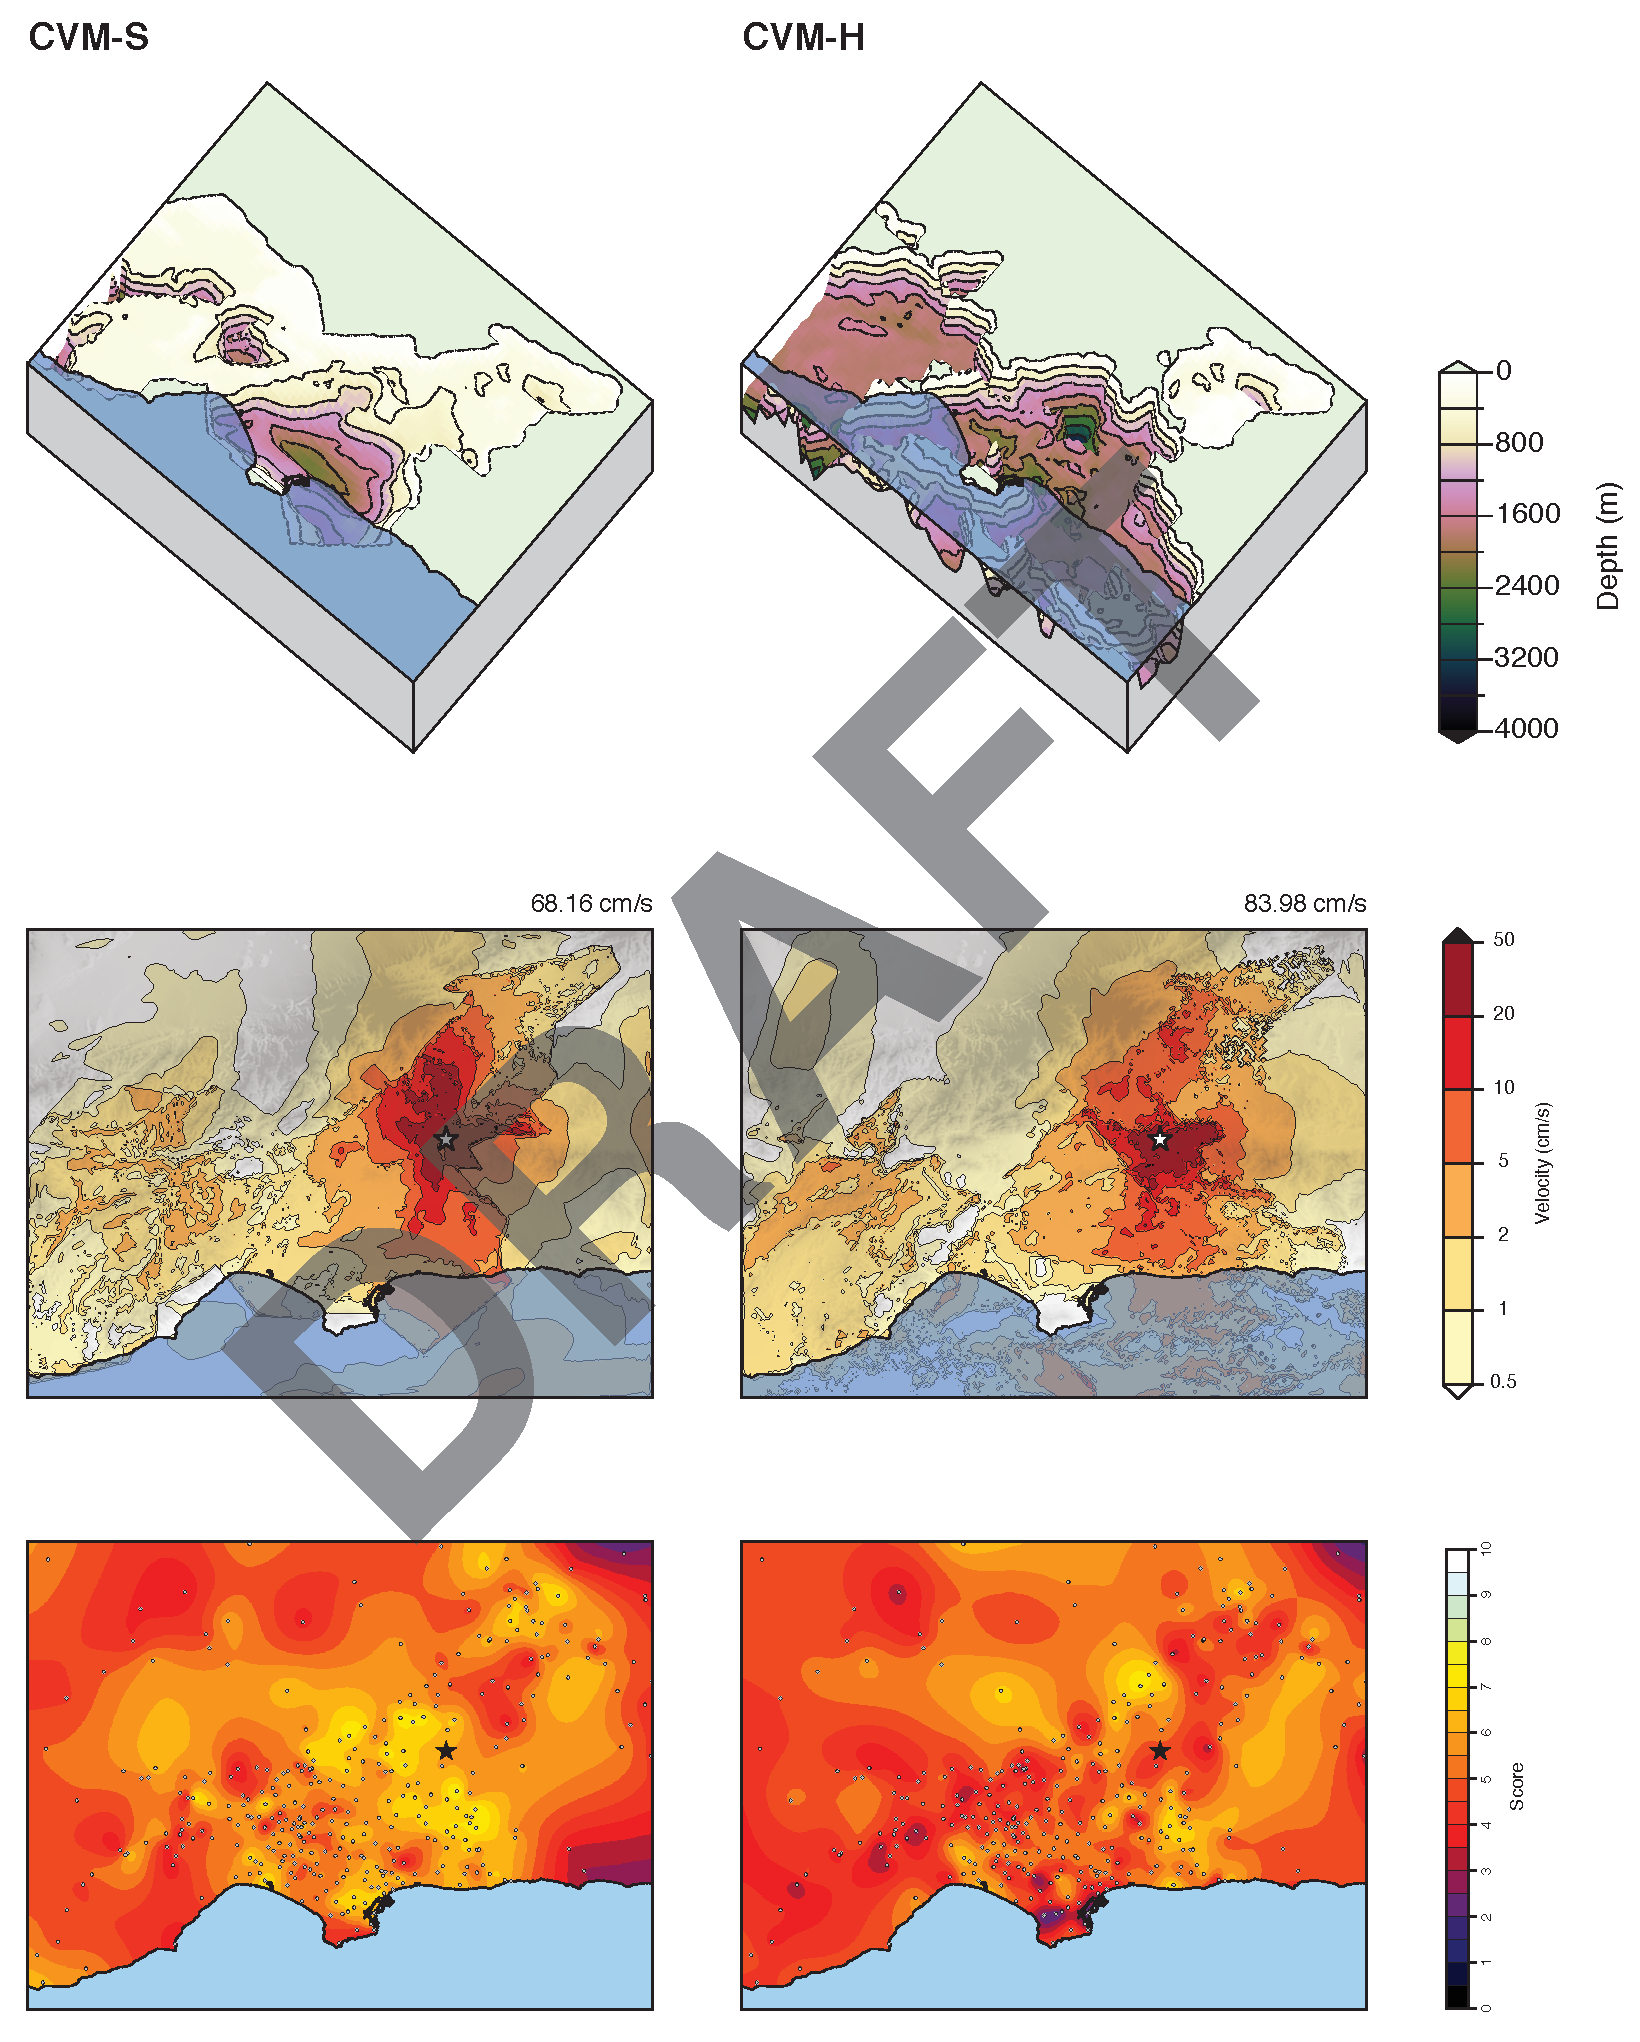
\includegraphics
		[width=0.75\textwidth]
		{figures/raw-pdf/ch-validation}
	\caption{\textcolor{red}{Temporary mock-up figure showing results from Chino Hills validation.}}
	\label{fig:ch.validation}
\end{figure*}
% ---------------------------------------------------------------------------------------------


\subsubsection{Effects of small-scale heterogeneities in simulation}
\label{sec:ch-ssh}

\textcolor{red}{I know the San Diego group did a series of simulations for Chino Hills in which they used SSH.  The caveat, though, is that they did those prior to SSH being implemented in UCVM.  Is there an alternative? If we have results using SSH as implemented in UCVM that are not Chino Hills, then we can simply move this up one level and present the Chino Hills results only from Hercules.}

\subsection{CyberShake}

\textcolor{red}{Desirable. I know there are results---preliminary, perhaps---if CyberShake using the different velocity models, and I presume the models used in the simulation where done using UCVM. Who would be the right person to help us prepare a text and a figure for this sub-section?}

\subsection{Something involving inversion and CVM-S4.26?}

\textcolor{red}{Tentative. I ignore the level of importance UCVM had on preparing the models for Po and En-Jui's inversions in preparation to obtain CVM-S4.26. I suppose that in any case, the fact that CVM-S-4.26 was produced and included in UCVM is something worth showcasing here. i will need, however, to think harder about how to put it in in a nice way.}

\subsection{Something involving the BBP?}

\textcolor{red}{Tentative. Is UCVM used at all in the BBP?}
